\documentclass[]{article}
\usepackage{lmodern}
\usepackage{amssymb,amsmath}
\usepackage{ifxetex,ifluatex}
\usepackage{fixltx2e} % provides \textsubscript
\ifnum 0\ifxetex 1\fi\ifluatex 1\fi=0 % if pdftex
  \usepackage[T1]{fontenc}
  \usepackage[utf8]{inputenc}
\else % if luatex or xelatex
  \ifxetex
    \usepackage{mathspec}
  \else
    \usepackage{fontspec}
  \fi
  \defaultfontfeatures{Ligatures=TeX,Scale=MatchLowercase}
\fi
% use upquote if available, for straight quotes in verbatim environments
\IfFileExists{upquote.sty}{\usepackage{upquote}}{}
% use microtype if available
\IfFileExists{microtype.sty}{%
\usepackage{microtype}
\UseMicrotypeSet[protrusion]{basicmath} % disable protrusion for tt fonts
}{}
\usepackage[margin=1in]{geometry}
\usepackage{hyperref}
\hypersetup{unicode=true,
            pdftitle={GREEN Grid Hot Water Profiles},
            pdfauthor={Ben Anderson (b.anderson@soton.ac.uk, @dataknut)},
            pdfborder={0 0 0},
            breaklinks=true}
\urlstyle{same}  % don't use monospace font for urls
\usepackage{color}
\usepackage{fancyvrb}
\newcommand{\VerbBar}{|}
\newcommand{\VERB}{\Verb[commandchars=\\\{\}]}
\DefineVerbatimEnvironment{Highlighting}{Verbatim}{commandchars=\\\{\}}
% Add ',fontsize=\small' for more characters per line
\usepackage{framed}
\definecolor{shadecolor}{RGB}{248,248,248}
\newenvironment{Shaded}{\begin{snugshade}}{\end{snugshade}}
\newcommand{\KeywordTok}[1]{\textcolor[rgb]{0.13,0.29,0.53}{\textbf{#1}}}
\newcommand{\DataTypeTok}[1]{\textcolor[rgb]{0.13,0.29,0.53}{#1}}
\newcommand{\DecValTok}[1]{\textcolor[rgb]{0.00,0.00,0.81}{#1}}
\newcommand{\BaseNTok}[1]{\textcolor[rgb]{0.00,0.00,0.81}{#1}}
\newcommand{\FloatTok}[1]{\textcolor[rgb]{0.00,0.00,0.81}{#1}}
\newcommand{\ConstantTok}[1]{\textcolor[rgb]{0.00,0.00,0.00}{#1}}
\newcommand{\CharTok}[1]{\textcolor[rgb]{0.31,0.60,0.02}{#1}}
\newcommand{\SpecialCharTok}[1]{\textcolor[rgb]{0.00,0.00,0.00}{#1}}
\newcommand{\StringTok}[1]{\textcolor[rgb]{0.31,0.60,0.02}{#1}}
\newcommand{\VerbatimStringTok}[1]{\textcolor[rgb]{0.31,0.60,0.02}{#1}}
\newcommand{\SpecialStringTok}[1]{\textcolor[rgb]{0.31,0.60,0.02}{#1}}
\newcommand{\ImportTok}[1]{#1}
\newcommand{\CommentTok}[1]{\textcolor[rgb]{0.56,0.35,0.01}{\textit{#1}}}
\newcommand{\DocumentationTok}[1]{\textcolor[rgb]{0.56,0.35,0.01}{\textbf{\textit{#1}}}}
\newcommand{\AnnotationTok}[1]{\textcolor[rgb]{0.56,0.35,0.01}{\textbf{\textit{#1}}}}
\newcommand{\CommentVarTok}[1]{\textcolor[rgb]{0.56,0.35,0.01}{\textbf{\textit{#1}}}}
\newcommand{\OtherTok}[1]{\textcolor[rgb]{0.56,0.35,0.01}{#1}}
\newcommand{\FunctionTok}[1]{\textcolor[rgb]{0.00,0.00,0.00}{#1}}
\newcommand{\VariableTok}[1]{\textcolor[rgb]{0.00,0.00,0.00}{#1}}
\newcommand{\ControlFlowTok}[1]{\textcolor[rgb]{0.13,0.29,0.53}{\textbf{#1}}}
\newcommand{\OperatorTok}[1]{\textcolor[rgb]{0.81,0.36,0.00}{\textbf{#1}}}
\newcommand{\BuiltInTok}[1]{#1}
\newcommand{\ExtensionTok}[1]{#1}
\newcommand{\PreprocessorTok}[1]{\textcolor[rgb]{0.56,0.35,0.01}{\textit{#1}}}
\newcommand{\AttributeTok}[1]{\textcolor[rgb]{0.77,0.63,0.00}{#1}}
\newcommand{\RegionMarkerTok}[1]{#1}
\newcommand{\InformationTok}[1]{\textcolor[rgb]{0.56,0.35,0.01}{\textbf{\textit{#1}}}}
\newcommand{\WarningTok}[1]{\textcolor[rgb]{0.56,0.35,0.01}{\textbf{\textit{#1}}}}
\newcommand{\AlertTok}[1]{\textcolor[rgb]{0.94,0.16,0.16}{#1}}
\newcommand{\ErrorTok}[1]{\textcolor[rgb]{0.64,0.00,0.00}{\textbf{#1}}}
\newcommand{\NormalTok}[1]{#1}
\usepackage{graphicx,grffile}
\makeatletter
\def\maxwidth{\ifdim\Gin@nat@width>\linewidth\linewidth\else\Gin@nat@width\fi}
\def\maxheight{\ifdim\Gin@nat@height>\textheight\textheight\else\Gin@nat@height\fi}
\makeatother
% Scale images if necessary, so that they will not overflow the page
% margins by default, and it is still possible to overwrite the defaults
% using explicit options in \includegraphics[width, height, ...]{}
\setkeys{Gin}{width=\maxwidth,height=\maxheight,keepaspectratio}
\IfFileExists{parskip.sty}{%
\usepackage{parskip}
}{% else
\setlength{\parindent}{0pt}
\setlength{\parskip}{6pt plus 2pt minus 1pt}
}
\setlength{\emergencystretch}{3em}  % prevent overfull lines
\providecommand{\tightlist}{%
  \setlength{\itemsep}{0pt}\setlength{\parskip}{0pt}}
\setcounter{secnumdepth}{5}
% Redefines (sub)paragraphs to behave more like sections
\ifx\paragraph\undefined\else
\let\oldparagraph\paragraph
\renewcommand{\paragraph}[1]{\oldparagraph{#1}\mbox{}}
\fi
\ifx\subparagraph\undefined\else
\let\oldsubparagraph\subparagraph
\renewcommand{\subparagraph}[1]{\oldsubparagraph{#1}\mbox{}}
\fi

%%% Use protect on footnotes to avoid problems with footnotes in titles
\let\rmarkdownfootnote\footnote%
\def\footnote{\protect\rmarkdownfootnote}

%%% Change title format to be more compact
\usepackage{titling}

% Create subtitle command for use in maketitle
\newcommand{\subtitle}[1]{
  \posttitle{
    \begin{center}\large#1\end{center}
    }
}

\setlength{\droptitle}{-2em}
  \title{GREEN Grid Hot Water Profiles}
  \pretitle{\vspace{\droptitle}\centering\huge}
  \posttitle{\par}
  \author{Ben Anderson
(\href{mailto:b.anderson@soton.ac.uk}{\nolinkurl{b.anderson@soton.ac.uk}},
\texttt{@dataknut})}
  \preauthor{\centering\large\emph}
  \postauthor{\par}
  \predate{\centering\large\emph}
  \postdate{\par}
  \date{Last run at: 2018-06-06 23:15:05}

\usepackage{booktabs}
\usepackage{longtable}
\usepackage{array}
\usepackage{multirow}
\usepackage[table]{xcolor}
\usepackage{wrapfig}
\usepackage{float}
\usepackage{colortbl}
\usepackage{pdflscape}
\usepackage{tabu}
\usepackage{threeparttable}
\usepackage{threeparttablex}
\usepackage[normalem]{ulem}
\usepackage{makecell}

\begin{document}
\maketitle

{
\setcounter{tocdepth}{2}
\tableofcontents
}
\newpage

\section{Status}\label{status}

Test run using reduced data from
\textasciitilde{}/Data/NZGreenGrid/gridspy/1min\_orig/

\section{Citation}\label{citation}

If you wish to use any of the material from this report please cite as:

\begin{itemize}
\tightlist
\item
  Anderson, B. (2018) GREEN Grid Hot Water Profiles, University of
  Otago: Dunedin, NZ.
\end{itemize}

\newpage

\section{Introduction}\label{introduction}

Report circulation:

\begin{itemize}
\tightlist
\item
  Restricted to:
  \href{https://www.otago.ac.nz/centre-sustainability/research/energy/otago050285.html}{NZ
  GREEN Grid} project partners and contractors.
\end{itemize}

\subsection{Purpose}\label{purpose}

This report is intended to:

\begin{itemize}
\tightlist
\item
  load and clean the project electricity power data (Grid Spy)
\item
  select the Hot Water circuits (via their labels)
\item
  build exploratory demand profiles
\end{itemize}

\subsection{Requirements:}\label{requirements}

\begin{itemize}
\tightlist
\item
  cleaned and safe grid spy 1 minute data processed via
  \url{https://git.soton.ac.uk/ba1e12/nzGREENGrid/blob/master/dataProcessing/processNZGGElecCons1minData.Rmd}
\end{itemize}

\subsection{History}\label{history}

Generally tracked via our git.soton
\href{https://git.soton.ac.uk/ba1e12/nzGREENGrid}{repo}:

\begin{itemize}
\tightlist
\item
  \href{https://git.soton.ac.uk/ba1e12/nzGREENGrid/commits/master}{history}
\item
  \href{https://git.soton.ac.uk/ba1e12/nzGREENGrid/issues}{issues}
\end{itemize}

\subsection{Support}\label{support}

This work was supported by:

\begin{itemize}
\tightlist
\item
  The \href{https://www.otago.ac.nz/}{University of Otago}
\item
  The New Zealand \href{http://www.mbie.govt.nz/}{Ministry of Business,
  Innovation and Employment (MBIE)}
\item
  \href{http://www.energy.soton.ac.uk/tag/spatialec/}{SPATIALEC} - a
  \href{http://ec.europa.eu/research/mariecurieactions/about-msca/actions/if/index_en.htm}{Marie
  Skłodowska-Curie Global Fellowship} based at the University of Otago's
  \href{http://www.otago.ac.nz/centre-sustainability/staff/otago673896.html}{Centre
  for Sustainability} (2017-2019) \& the University of Southampton's
  Sustainable Energy Research Group (2019-202).
\end{itemize}

This work is (c) 2018 the University of Southampton.

We do not `support' the code but if you have a problem check the
\href{https://git.soton.ac.uk/ba1e12/nzGREENGrid/issues}{issues} on our
\href{https://git.soton.ac.uk/ba1e12/nzGREENGrid}{repo} and if it
doesn't already exist, open one. We might be able to fix it :-)

\section{Load data files}\label{load-data-files}

\subsection{Grid Spy metadata}\label{grid-spy-metadata}

In this section we load metadata from /Users/ben/Syncplicity
Folders/Green Grid Project Management Folder/Gridspy/Master list of
Gridspy units.xlsx to link to the power data.

\begin{verbatim}
##    sample  hhID          Adults Teenagers             Children removed
## 1: Unison rf_28               2      <NA>            3(12,8,4)    <NA>
## 2: Unison rf_29               2      <NA>     1 (7 months old)    live
## 3: Unison rf_30               2         0                    0    <NA>
## 4: Unison rf_31 2 (Plus cousin)      <NA>                 <NA>    live
## 5: Unison rf_32               2      <NA> 2 (7 and 4years old)    <NA>
## 6: Unison rf_33               2 1(14yold)            1 (6yold)    live
\end{verbatim}

\begin{verbatim}
##     sample  hhID Adults Teenagers Children  removed
## 1: Powerco rf_12      1      <NA>     <NA> 3/6/1015
## 2: Powerco  <NA>      1      <NA>     <NA>     <NA>
## 3: Powerco rf_25      1      <NA>     <NA>     <NA>
## 4: Powerco  <NA>     NA      <NA>     <NA>     <NA>
## 5: Powerco  <NA>      1      <NA>   1(5mo)     <NA>
## 6: Powerco  <NA>     NA      <NA>     <NA>     <NA>
\end{verbatim}

\begin{table}

\caption{\label{tab:load metadata}Meta data for sample}
\centering
\begin{tabular}[t]{l|l|l|l|l|l|l}
\hline
sample & hhID & Adults & Teenagers & Children & removed & nAdults\\
\hline
Powerco & rf\_06 & 2 & NA & NA & NA & 2\\
\hline
Powerco & rf\_07 & 2 & NA & 2 & NA & 2\\
\hline
Powerco & rf\_08 & 2 & NA & NA & NA & 2\\
\hline
Powerco & rf\_09 & 2 & NA & 1 & 42171 & 2\\
\hline
Powerco & rf\_10 & 2 & NA & 1(3yo) & NA & 3\\
\hline
Powerco & rf\_11 & NA & NA & NA & NA & 1\\
\hline
Powerco & rf\_12 & 1 & NA & NA & 3/6/1015 & 1\\
\hline
Powerco & rf\_13 & 2 & 1(16yo) & 1(11) & NA & 2\\
\hline
Powerco & rf\_14 & 1 & NA & 1 (11 yo) & NA & 1\\
\hline
Powerco & rf\_15 & NA & NA & NA & 42462 & 1\\
\hline
Powerco & rf\_15\_old & 1 & NA & NA & 42019 & 1\\
\hline
Powerco & rf\_16 & 2 & NA & NA & 42089 & 2\\
\hline
Powerco & rf\_17 sn\_662 & NA & NA & NA & NA & 1\\
\hline
Powerco & rf\_17\_oldNo reused & 2 & 1(13yo) & 1(11yo) & 42457 & 2\\
\hline
Powerco & rf\_18 & 2 & NA & 1(1yo) & 42532 & 2\\
\hline
Powerco & rf\_19 & 1 & NA & NA & NA & 1\\
\hline
Powerco & rf\_20 & 2 & NA & 2 & 42166 & 2\\
\hline
Powerco & rf\_21 & 2 & NA & NA & 42821 & 2\\
\hline
Powerco & rf\_22 & 2 & NA & NA & NA & 2\\
\hline
Powerco & rf\_23 & 1 & NA & NA & NA & 1\\
\hline
Powerco & rf\_24 & 2 & NA & 2 & NA & 2\\
\hline
Powerco & rf\_25 & 1 & NA & NA & NA & 1\\
\hline
Powerco & rf\_26 & 2 & NA & NA & NA & 2\\
\hline
Powerco & rf\_27 & 2 & 1 & 1 & NA & 2\\
\hline
Unison & rf\_28 & 2 & NA & 3(12,8,4) & NA & 3\\
\hline
Unison & rf\_29 & 2 & NA & 1 (7 months old) & live & 2\\
\hline
Unison & rf\_30 & 2 & 0 & 0 & NA & 2\\
\hline
Unison & rf\_31 & 2 (Plus cousin) & NA & NA & live & 2\\
\hline
Unison & rf\_32 & 2 & NA & 2 (7 and 4years old) & NA & 2\\
\hline
Unison & rf\_33 & 2 & 1(14yold) & 1 (6yold) & live & 2\\
\hline
Unison & rf\_34 & 3 & NA & NA & NA & 1\\
\hline
Unison & rf\_35 & 2 & NA & NA & 42322 & 2\\
\hline
Unison & rf\_36 & 1 & 2 (14 and 12) & NA & live & 1\\
\hline
Unison & rf\_37 & 2 & NA & NA & live & 2\\
\hline
Unison & rf\_38 & NA & NA & NA & NA & 1\\
\hline
Unison & rf\_38 & 2 & NA & 2 (<12) & NA & 2\\
\hline
Unison & rf\_39 & 2 & 1 (16 YO) & NA & live & 2\\
\hline
Unison & rf\_40 & 2 & NA & NA & 42330 & 2\\
\hline
Unison & rf\_41 & 2 & NA & 2 (11 and 8) & live & 2\\
\hline
Unison & rf\_42 & 2 & NA & 3 (<12 yold, 1 10 YO) & NA & 3\\
\hline
Unison & rf\_43 & 2 & NA & NA & 42296 & 2\\
\hline
Unison & rf\_44 & 2 & NA & 2 (10 and 7) & NA & 2\\
\hline
Unison & rf\_45 & 2 & NA & 3 (<12 years old) & NA & 3\\
\hline
Unison & rf\_46 & 2 & NA & 1 (4yold-50\%) & live & 2\\
\hline
Unison & rf\_47 & 3 & 2 & NA & NA & 1\\
\hline
\end{tabular}
\end{table}

\subsection{Grid Spy data}\label{grid-spy-data}

In this section we load the cleaned data files from
\textasciitilde{}/Data/NZGreenGrid/safe/gridSpy/1min/data/. If we loaded
all the data at once and then filtered out what we want we might run out
of memory so we filter as we load. Set the filters here:

\begin{Shaded}
\begin{Highlighting}[]
\NormalTok{circuitPattern <-}\StringTok{ "Hot Water"}
\NormalTok{dateFrom <-}\StringTok{ "2015-04-01"}
\NormalTok{dateTo <-}\StringTok{ "2016-03-31"}

\NormalTok{plotCaption <-}\StringTok{ }\KeywordTok{paste0}\NormalTok{(}\StringTok{"Source: "}\NormalTok{, fpath,}
                      \StringTok{"}\CharTok{\textbackslash{}n}\StringTok{Circuits: "}\NormalTok{, circuitPattern, }\StringTok{" from "}\NormalTok{, dateFrom, }\StringTok{" to "}\NormalTok{, dateTo)}
\end{Highlighting}
\end{Shaded}

So we are looking for Hot Water circuits between 2015-04-01 and
2016-03-31. We do this by checking to see if the extract file has
already been created. If so we load it. If not, we create it.

The file we are looking for is: Hot
Water\_2015-04-01\_2016-03-31\_observations.csv

\begin{verbatim}
## [1] "~/Data/NZGreenGrid/safe/gridSpy/1min/dataExtracts/Hot Water_2015-04-01_2016-03-31_observations.csv exists so re-loading..."
## [1] "# Loaded 14,496,831 rows of data"
\end{verbatim}

The following table summarises the Hot Water data we have found.

\begin{table}

\caption{\label{tab:sumamrise loaded data}Summary of household grid spy data for: Hot Water}
\centering
\begin{tabular}[t]{l|r|r|r|r|l|l}
\hline
hhID & nObs & nHouseholds & nCircuits & meanPower & minDate & maxDate\\
\hline
rf\_02 & 81647 & 1 & 1 & 390.7312904 & 2015-04-01 & 2015-05-28\\
\hline
rf\_06 & 523312 & 1 & 1 & 387.3524992 & 2015-04-01 & 2016-03-31\\
\hline
rf\_08 & 521843 & 1 & 1 & 307.4189980 & 2015-04-01 & 2016-03-31\\
\hline
rf\_11 & 519185 & 1 & 1 & 67.1572238 & 2015-04-01 & 2016-03-31\\
\hline
rf\_12 & 80081 & 1 & 1 & 418.5545972 & 2015-04-01 & 2015-06-02\\
\hline
rf\_13 & 526929 & 1 & 1 & 152.3181436 & 2015-04-01 & 2016-03-31\\
\hline
rf\_14 & 525470 & 1 & 1 & 235.1927161 & 2015-04-01 & 2016-03-31\\
\hline
rf\_15 & 273252 & 1 & 1 & 448.6198651 & 2015-04-01 & 2015-11-28\\
\hline
rf\_17 & 520028 & 1 & 1 & 0.0002596 & 2015-04-01 & 2016-03-28\\
\hline
rf\_18 & 102202 & 1 & 1 & 390.3190006 & 2015-04-01 & 2015-06-11\\
\hline
rf\_20 & 102188 & 1 & 1 & 292.2748598 & 2015-04-01 & 2015-06-11\\
\hline
rf\_22 & 526097 & 1 & 1 & 530.7474282 & 2015-04-01 & 2016-03-31\\
\hline
rf\_23 & 519906 & 1 & 1 & 206.0260549 & 2015-04-01 & 2016-03-31\\
\hline
rf\_24 & 520556 & 1 & 1 & 478.1132036 & 2015-04-01 & 2016-03-31\\
\hline
rf\_25 & 443936 & 1 & 1 & 230.5553235 & 2015-05-24 & 2016-03-31\\
\hline
rf\_27 & 497806 & 1 & 1 & 137.8961919 & 2015-04-01 & 2016-03-31\\
\hline
rf\_29 & 526780 & 1 & 1 & 358.8502211 & 2015-04-01 & 2016-03-31\\
\hline
rf\_30 & 477491 & 1 & 1 & 194.0280348 & 2015-04-01 & 2016-03-31\\
\hline
rf\_31 & 526878 & 1 & 1 & 194.3654428 & 2015-04-01 & 2016-03-31\\
\hline
rf\_32 & 526785 & 1 & 1 & 284.6575412 & 2015-04-01 & 2016-03-31\\
\hline
rf\_33 & 526863 & 1 & 1 & 326.9971683 & 2015-04-01 & 2016-03-31\\
\hline
rf\_34 & 526677 & 1 & 1 & 319.3515297 & 2015-04-01 & 2016-03-31\\
\hline
rf\_35 & 327974 & 1 & 1 & 251.4110126 & 2015-04-01 & 2015-11-14\\
\hline
rf\_36 & 516242 & 1 & 1 & 262.2140651 & 2015-04-01 & 2016-03-31\\
\hline
rf\_37 & 526771 & 1 & 1 & 344.2228600 & 2015-04-01 & 2016-03-31\\
\hline
rf\_38 & 373722 & 1 & 1 & 472.3660753 & 2015-04-01 & 2015-12-26\\
\hline
rf\_39 & 495806 & 1 & 1 & 377.7922476 & 2015-04-01 & 2016-03-31\\
\hline
rf\_40 & 338289 & 1 & 1 & 338.7696737 & 2015-04-01 & 2015-11-22\\
\hline
rf\_42 & 518179 & 1 & 1 & 377.6124709 & 2015-04-01 & 2016-03-31\\
\hline
rf\_44 & 526850 & 1 & 1 & 463.7929726 & 2015-04-01 & 2016-03-31\\
\hline
rf\_45 & 526110 & 1 & 1 & 300.3924577 & 2015-04-01 & 2016-03-31\\
\hline
rf\_46 & 950976 & 1 & 2 & 102.9197503 & 2015-04-01 & 2016-03-31\\
\hline
\end{tabular}
\end{table}

This table will have a large number (14,496,831) of obserations caused
by the number of different circuit labels as shown by the following
table.

\begin{table}

\caption{\label{tab:test circuit labels}Counts of Hot Water observations by label and household}
\centering
\begin{tabular}[t]{l|r|r|r|r|r|r|r|r|r|r|r|r|r|r|r|r|r|r|r|r|r|r|r|r|r|r|r|r|r|r|r|r}
\hline
  & rf\_02 & rf\_06 & rf\_08 & rf\_11 & rf\_12 & rf\_13 & rf\_14 & rf\_15 & rf\_17 & rf\_18 & rf\_20 & rf\_22 & rf\_23 & rf\_24 & rf\_25 & rf\_27 & rf\_29 & rf\_30 & rf\_31 & rf\_32 & rf\_33 & rf\_34 & rf\_35 & rf\_36 & rf\_37 & rf\_38 & rf\_39 & rf\_40 & rf\_42 & rf\_44 & rf\_45 & rf\_46\\
\hline
Hot Water  (2 elements)\$4247 & 0 & 0 & 0 & 0 & 0 & 0 & 0 & 0 & 0 & 0 & 0 & 0 & 0 & 0 & 0 & 0 & 0 & 0 & 0 & 0 & 0 & 0 & 0 & 0 & 0 & 0 & 495806 & 0 & 0 & 0 & 0 & 0\\
\hline
Hot Water - Controlled (HEMS)\$2081 & 0 & 0 & 0 & 0 & 0 & 0 & 0 & 0 & 0 & 0 & 0 & 0 & 519906 & 0 & 0 & 0 & 0 & 0 & 0 & 0 & 0 & 0 & 0 & 0 & 0 & 0 & 0 & 0 & 0 & 0 & 0 & 0\\
\hline
Hot Water - Controlled\$2094 & 0 & 0 & 521843 & 0 & 0 & 0 & 0 & 0 & 0 & 0 & 0 & 0 & 0 & 0 & 0 & 0 & 0 & 0 & 0 & 0 & 0 & 0 & 0 & 0 & 0 & 0 & 0 & 0 & 0 & 0 & 0 & 0\\
\hline
Hot Water - Controlled\$2102 & 0 & 0 & 0 & 0 & 0 & 0 & 0 & 0 & 0 & 0 & 0 & 0 & 0 & 520556 & 0 & 0 & 0 & 0 & 0 & 0 & 0 & 0 & 0 & 0 & 0 & 0 & 0 & 0 & 0 & 0 & 0 & 0\\
\hline
Hot Water - Controlled\$2110 & 0 & 0 & 0 & 0 & 0 & 0 & 0 & 0 & 0 & 0 & 102188 & 0 & 0 & 0 & 0 & 0 & 0 & 0 & 0 & 0 & 0 & 0 & 0 & 0 & 0 & 0 & 0 & 0 & 0 & 0 & 0 & 0\\
\hline
Hot Water - Controlled\$2129 & 0 & 0 & 0 & 0 & 0 & 0 & 0 & 0 & 0 & 102202 & 0 & 0 & 0 & 0 & 0 & 0 & 0 & 0 & 0 & 0 & 0 & 0 & 0 & 0 & 0 & 0 & 0 & 0 & 0 & 0 & 0 & 0\\
\hline
Hot Water - Controlled\$2150 & 0 & 0 & 0 & 0 & 0 & 0 & 0 & 0 & 520028 & 0 & 0 & 0 & 0 & 0 & 0 & 0 & 0 & 0 & 0 & 0 & 0 & 0 & 0 & 0 & 0 & 0 & 0 & 0 & 0 & 0 & 0 & 0\\
\hline
Hot Water - Controlled\$2208 & 0 & 0 & 0 & 0 & 0 & 526929 & 0 & 0 & 0 & 0 & 0 & 0 & 0 & 0 & 0 & 0 & 0 & 0 & 0 & 0 & 0 & 0 & 0 & 0 & 0 & 0 & 0 & 0 & 0 & 0 & 0 & 0\\
\hline
Hot Water - Controlled\$2236 & 0 & 0 & 0 & 0 & 0 & 0 & 0 & 0 & 0 & 0 & 0 & 526097 & 0 & 0 & 0 & 0 & 0 & 0 & 0 & 0 & 0 & 0 & 0 & 0 & 0 & 0 & 0 & 0 & 0 & 0 & 0 & 0\\
\hline
Hot Water - Controlled\$2248 & 0 & 523312 & 0 & 0 & 0 & 0 & 0 & 0 & 0 & 0 & 0 & 0 & 0 & 0 & 0 & 0 & 0 & 0 & 0 & 0 & 0 & 0 & 0 & 0 & 0 & 0 & 0 & 0 & 0 & 0 & 0 & 0\\
\hline
Hot Water - Controlled\$2719 & 0 & 0 & 0 & 0 & 0 & 0 & 525470 & 0 & 0 & 0 & 0 & 0 & 0 & 0 & 0 & 0 & 0 & 0 & 0 & 0 & 0 & 0 & 0 & 0 & 0 & 0 & 0 & 0 & 0 & 0 & 0 & 0\\
\hline
Hot Water - Controlled\$2761 & 0 & 0 & 0 & 0 & 0 & 0 & 0 & 0 & 0 & 0 & 0 & 0 & 0 & 0 & 443936 & 0 & 0 & 0 & 0 & 0 & 0 & 0 & 0 & 0 & 0 & 0 & 0 & 0 & 0 & 0 & 0 & 0\\
\hline
Hot Water - Controlled\$2825 & 0 & 0 & 0 & 0 & 0 & 0 & 0 & 0 & 0 & 0 & 0 & 0 & 0 & 0 & 0 & 497806 & 0 & 0 & 0 & 0 & 0 & 0 & 0 & 0 & 0 & 0 & 0 & 0 & 0 & 0 & 0 & 0\\
\hline
Hot Water - Controlled\$4135 & 0 & 0 & 0 & 0 & 0 & 0 & 0 & 0 & 0 & 0 & 0 & 0 & 0 & 0 & 0 & 0 & 0 & 0 & 0 & 0 & 0 & 0 & 0 & 0 & 526771 & 0 & 0 & 0 & 0 & 0 & 0 & 0\\
\hline
Hot Water - Controlled\$4144 & 0 & 0 & 0 & 0 & 0 & 0 & 0 & 0 & 0 & 0 & 0 & 0 & 0 & 0 & 0 & 0 & 0 & 0 & 0 & 0 & 526863 & 0 & 0 & 0 & 0 & 0 & 0 & 0 & 0 & 0 & 0 & 0\\
\hline
Hot Water - Controlled\$4155 & 0 & 0 & 0 & 0 & 0 & 0 & 0 & 0 & 0 & 0 & 0 & 0 & 0 & 0 & 0 & 0 & 0 & 0 & 0 & 0 & 0 & 0 & 0 & 0 & 0 & 0 & 0 & 0 & 0 & 526850 & 0 & 0\\
\hline
Hot Water - Controlled\$4158 & 0 & 0 & 0 & 0 & 0 & 0 & 0 & 0 & 0 & 0 & 0 & 0 & 0 & 0 & 0 & 0 & 0 & 0 & 0 & 0 & 0 & 0 & 0 & 0 & 0 & 0 & 0 & 0 & 0 & 0 & 526110 & 0\\
\hline
Hot Water - Controlled\$4167 & 0 & 0 & 0 & 0 & 0 & 0 & 0 & 0 & 0 & 0 & 0 & 0 & 0 & 0 & 0 & 0 & 0 & 0 & 0 & 0 & 0 & 0 & 0 & 0 & 0 & 0 & 0 & 338289 & 0 & 0 & 0 & 0\\
\hline
Hot Water - Controlled\$4178 & 0 & 0 & 0 & 0 & 0 & 0 & 0 & 0 & 0 & 0 & 0 & 0 & 0 & 0 & 0 & 0 & 0 & 0 & 0 & 0 & 0 & 0 & 0 & 0 & 0 & 373722 & 0 & 0 & 0 & 0 & 0 & 0\\
\hline
Hot Water - Controlled\$4184 & 0 & 0 & 0 & 0 & 0 & 0 & 0 & 0 & 0 & 0 & 0 & 0 & 0 & 0 & 0 & 0 & 526780 & 0 & 0 & 0 & 0 & 0 & 0 & 0 & 0 & 0 & 0 & 0 & 0 & 0 & 0 & 0\\
\hline
Hot Water - Controlled\$4198 & 0 & 0 & 0 & 0 & 0 & 0 & 0 & 0 & 0 & 0 & 0 & 0 & 0 & 0 & 0 & 0 & 0 & 0 & 0 & 526785 & 0 & 0 & 0 & 0 & 0 & 0 & 0 & 0 & 0 & 0 & 0 & 0\\
\hline
Hot Water - Controlled\$4200 & 0 & 0 & 0 & 0 & 0 & 0 & 0 & 0 & 0 & 0 & 0 & 0 & 0 & 0 & 0 & 0 & 0 & 0 & 526878 & 0 & 0 & 0 & 0 & 0 & 0 & 0 & 0 & 0 & 0 & 0 & 0 & 0\\
\hline
Hot Water - Controlled\$4231 & 0 & 0 & 0 & 0 & 0 & 0 & 0 & 0 & 0 & 0 & 0 & 0 & 0 & 0 & 0 & 0 & 0 & 0 & 0 & 0 & 0 & 0 & 0 & 0 & 0 & 0 & 0 & 0 & 0 & 0 & 0 & 486982\\
\hline
Hot Water - Controlled\$4238 & 0 & 0 & 0 & 0 & 0 & 0 & 0 & 0 & 0 & 0 & 0 & 0 & 0 & 0 & 0 & 0 & 0 & 477491 & 0 & 0 & 0 & 0 & 0 & 0 & 0 & 0 & 0 & 0 & 0 & 0 & 0 & 0\\
\hline
Hot Water - Controlled\$4400 & 0 & 0 & 0 & 0 & 0 & 0 & 0 & 0 & 0 & 0 & 0 & 0 & 0 & 0 & 0 & 0 & 0 & 0 & 0 & 0 & 0 & 0 & 0 & 0 & 0 & 0 & 0 & 0 & 0 & 0 & 0 & 463994\\
\hline
Hot Water - Uncontrolled\$4125 & 0 & 0 & 0 & 0 & 0 & 0 & 0 & 0 & 0 & 0 & 0 & 0 & 0 & 0 & 0 & 0 & 0 & 0 & 0 & 0 & 0 & 0 & 327974 & 0 & 0 & 0 & 0 & 0 & 0 & 0 & 0 & 0\\
\hline
Hot Water - Uncontrolled\$4131 & 0 & 0 & 0 & 0 & 0 & 0 & 0 & 0 & 0 & 0 & 0 & 0 & 0 & 0 & 0 & 0 & 0 & 0 & 0 & 0 & 0 & 0 & 0 & 0 & 0 & 0 & 0 & 0 & 518179 & 0 & 0 & 0\\
\hline
Hot Water - Uncontrolled\$4147 & 0 & 0 & 0 & 0 & 0 & 0 & 0 & 0 & 0 & 0 & 0 & 0 & 0 & 0 & 0 & 0 & 0 & 0 & 0 & 0 & 0 & 0 & 0 & 516242 & 0 & 0 & 0 & 0 & 0 & 0 & 0 & 0\\
\hline
Hot Water - Uncontrolled\$4224 & 0 & 0 & 0 & 0 & 0 & 0 & 0 & 0 & 0 & 0 & 0 & 0 & 0 & 0 & 0 & 0 & 0 & 0 & 0 & 0 & 0 & 526677 & 0 & 0 & 0 & 0 & 0 & 0 & 0 & 0 & 0 & 0\\
\hline
Hot Water Cpbd Heater- Cont\$2586 & 0 & 0 & 0 & 519185 & 0 & 0 & 0 & 0 & 0 & 0 & 0 & 0 & 0 & 0 & 0 & 0 & 0 & 0 & 0 & 0 & 0 & 0 & 0 & 0 & 0 & 0 & 0 & 0 & 0 & 0 & 0 & 0\\
\hline
Hot Water\$1574 & 81647 & 0 & 0 & 0 & 0 & 0 & 0 & 0 & 0 & 0 & 0 & 0 & 0 & 0 & 0 & 0 & 0 & 0 & 0 & 0 & 0 & 0 & 0 & 0 & 0 & 0 & 0 & 0 & 0 & 0 & 0 & 0\\
\hline
Hot Water\$3952 & 0 & 0 & 0 & 0 & 0 & 0 & 0 & 273252 & 0 & 0 & 0 & 0 & 0 & 0 & 0 & 0 & 0 & 0 & 0 & 0 & 0 & 0 & 0 & 0 & 0 & 0 & 0 & 0 & 0 & 0 & 0 & 0\\
\hline
Incomer 1 - Hot Water - Cont\$2626 & 0 & 0 & 0 & 0 & 80081 & 0 & 0 & 0 & 0 & 0 & 0 & 0 & 0 & 0 & 0 & 0 & 0 & 0 & 0 & 0 & 0 & 0 & 0 & 0 & 0 & 0 & 0 & 0 & 0 & 0 & 0 & 0\\
\hline
\end{tabular}
\end{table}

Note that some households may have more than one Hot Water circuit.

\subsection{Test Hot Water data}\label{test-hot-water-data}

This section tests the availability of Hot Water data by replicating the
standard data quality checks used for the whole
\href{https://git.soton.ac.uk/ba1e12/nzGREENGrid/tree/master/dataProcessing/gridSpy}{gridSpy
dataset}.

The following plot shows loaded data observation plots - just to confirm
what Hot Water data we have.

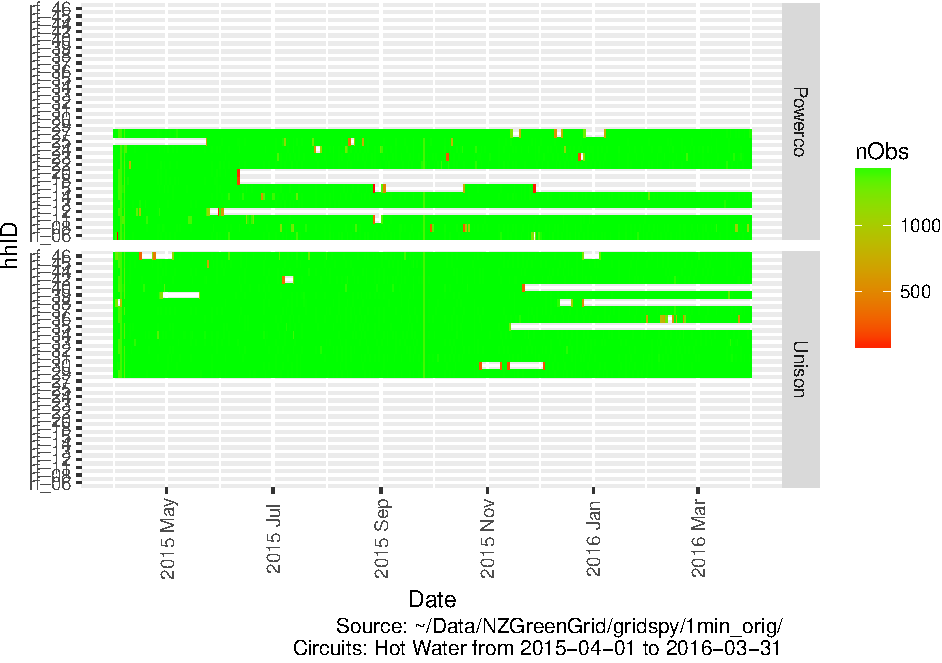
\includegraphics{ggHotWaterProfiles_files/figure-latex/loadedFilesObs Tile Plot-1.pdf}

The next plot shows the same data but as a dot plot to highlight those
households and dates where we did not receive 60 * 24 = 1440
observations per day.

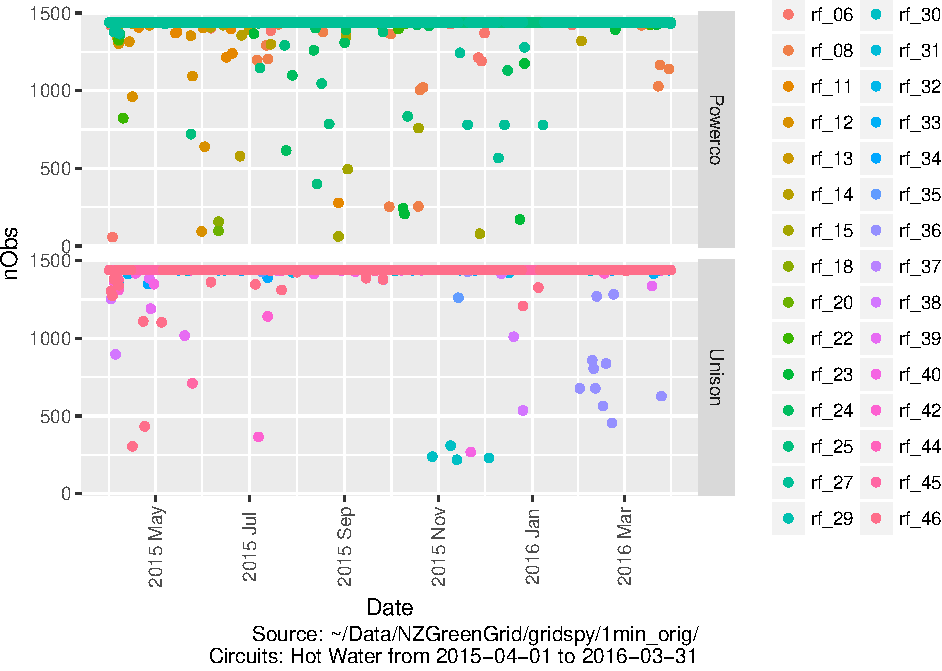
\includegraphics{ggHotWaterProfiles_files/figure-latex/loadedFilesObs point plot-1.pdf}

The following table shows the min/max observations per day and min/max
dates for each household. As above, we should not see:

\begin{itemize}
\tightlist
\item
  dates before 2014 or in to the future (indicates date conversion
  errors)
\item
  more than 1440 observations per day (indicates potentially duplicate
  observations)
\item
  non-integer counts of circuits as it suggests some column errors
\end{itemize}

We should also not see NA in any row (indicates date conversion errors).

If we do see any of these then we still have data cleaning work to do!

\begin{table}

\caption{\label{tab:summaryTable}Summary observation stats by hhID (sorted by date last heard from) for: Hot Water}
\centering
\begin{tabular}[t]{l|l|r|l|l}
\hline
hhID & sample & nObs & minDate & maxDate\\
\hline
rf\_12 & Powerco & 80081 & 2015-04-01T00:00:00Z & 2015-06-02T20:07:00Z\\
\hline
rf\_20 & Powerco & 102188 & 2015-04-01T00:00:00Z & 2015-06-11T01:37:00Z\\
\hline
rf\_18 & Powerco & 102202 & 2015-04-01T00:00:00Z & 2015-06-11T02:36:00Z\\
\hline
rf\_35 & Unison & 327974 & 2015-04-01T00:00:00Z & 2015-11-14T21:00:00Z\\
\hline
rf\_40 & Unison & 338289 & 2015-04-01T00:00:00Z & 2015-11-22T04:27:00Z\\
\hline
rf\_15 & Powerco & 273252 & 2015-04-01T00:00:00Z & 2015-11-28T01:19:00Z\\
\hline
rf\_38 & Unison & 747444 & 2015-04-01T00:00:00Z & 2015-12-26T08:55:00Z\\
\hline
rf\_06 & Powerco & 523312 & 2015-04-01T00:00:00Z & 2016-03-31T23:59:00Z\\
\hline
rf\_08 & Powerco & 521843 & 2015-04-01T00:00:00Z & 2016-03-31T23:59:00Z\\
\hline
rf\_11 & Powerco & 519185 & 2015-04-01T00:00:00Z & 2016-03-31T23:59:00Z\\
\hline
rf\_13 & Powerco & 526929 & 2015-04-01T00:00:00Z & 2016-03-31T23:59:00Z\\
\hline
rf\_14 & Powerco & 525470 & 2015-04-01T00:00:00Z & 2016-03-31T23:59:00Z\\
\hline
rf\_22 & Powerco & 526097 & 2015-04-01T00:00:00Z & 2016-03-31T23:59:00Z\\
\hline
rf\_23 & Powerco & 519906 & 2015-04-01T00:00:00Z & 2016-03-31T23:59:00Z\\
\hline
rf\_24 & Powerco & 520556 & 2015-04-01T00:00:00Z & 2016-03-31T23:59:00Z\\
\hline
rf\_25 & Powerco & 443936 & 2015-05-24T12:00:00Z & 2016-03-31T23:59:00Z\\
\hline
rf\_27 & Powerco & 497806 & 2015-04-01T00:00:00Z & 2016-03-31T23:59:00Z\\
\hline
rf\_29 & Unison & 526780 & 2015-04-01T00:00:00Z & 2016-03-31T23:59:00Z\\
\hline
rf\_30 & Unison & 477491 & 2015-04-01T00:00:00Z & 2016-03-31T23:59:00Z\\
\hline
rf\_31 & Unison & 526878 & 2015-04-01T00:00:00Z & 2016-03-31T23:59:00Z\\
\hline
rf\_32 & Unison & 526785 & 2015-04-01T00:00:00Z & 2016-03-31T23:59:00Z\\
\hline
rf\_33 & Unison & 526863 & 2015-04-01T00:00:00Z & 2016-03-31T23:59:00Z\\
\hline
rf\_34 & Unison & 526677 & 2015-04-01T00:00:00Z & 2016-03-31T23:59:00Z\\
\hline
rf\_36 & Unison & 516242 & 2015-04-01T00:00:00Z & 2016-03-31T23:59:00Z\\
\hline
rf\_37 & Unison & 526771 & 2015-04-01T00:00:00Z & 2016-03-31T23:59:00Z\\
\hline
rf\_39 & Unison & 495806 & 2015-04-01T00:00:00Z & 2016-03-31T23:59:00Z\\
\hline
rf\_42 & Unison & 518179 & 2015-04-01T00:00:00Z & 2016-03-31T23:59:00Z\\
\hline
rf\_44 & Unison & 526850 & 2015-04-01T00:00:00Z & 2016-03-31T23:59:00Z\\
\hline
rf\_45 & Unison & 526110 & 2015-04-01T00:00:00Z & 2016-03-31T23:59:00Z\\
\hline
rf\_46 & Unison & 950976 & 2015-04-01T00:00:00Z & 2016-03-31T23:59:00Z\\
\hline
\end{tabular}
\end{table}

Finally we show the total number of households which we think we have
Hot Water data for.

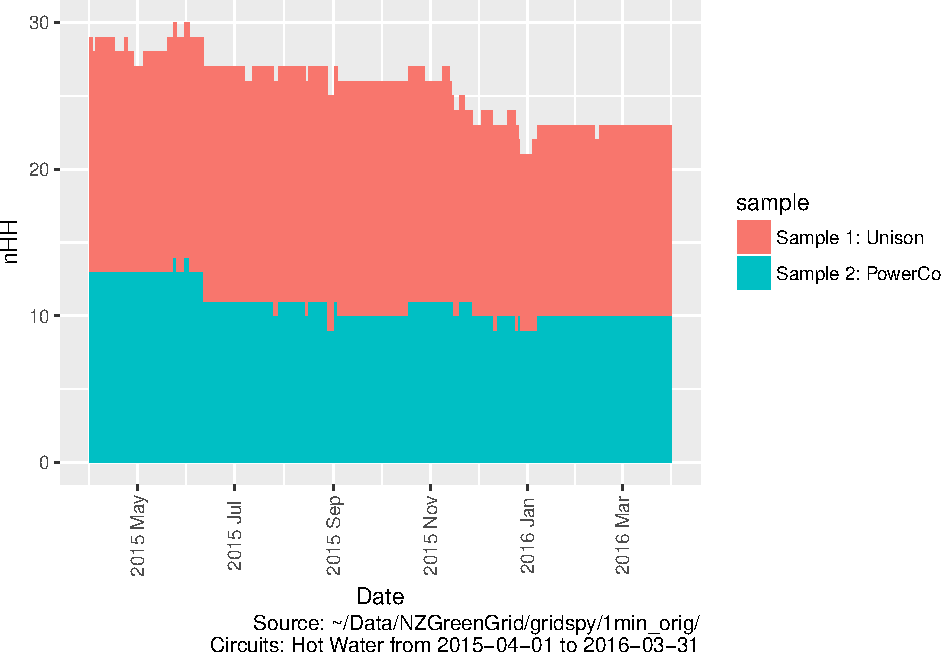
\includegraphics{ggHotWaterProfiles_files/figure-latex/liveDataHouseholds-1.pdf}

The following table summarises the Hot Water data. Any surprises?

\begin{Shaded}
\begin{Highlighting}[]
\NormalTok{t <-}\StringTok{ }\KeywordTok{summary}\NormalTok{(gs1MinDT)}
\KeywordTok{kable}\NormalTok{(}\DataTypeTok{caption =} \KeywordTok{paste0}\NormalTok{(}\StringTok{"Summary of "}\NormalTok{, circuitPattern, }\StringTok{" circuits"}\NormalTok{), t)}
\end{Highlighting}
\end{Shaded}

\begin{table}

\caption{\label{tab:summary of cols}Summary of Hot Water circuits}
\centering
\begin{tabular}[t]{l|l|l|l|l|l}
\hline
  &     hhID &  r\_dateTime &   circuit &     powerW &  obsHourMin\\
\hline
 & Length:14496831 & Length:14496831 & Length:14496831 & Min.   :-1110.0 & Length:14496831\\
\hline
 & Class :character & Class :character & Class :character & 1st Qu.:    0.0 & Class :character\\
\hline
 & Mode  :character & Mode  :character & Mode  :character & Median :    0.0 & Mode  :character\\
\hline
 & NA & NA & NA & Mean   :  283.8 & NA\\
\hline
 & NA & NA & NA & 3rd Qu.:    0.0 & NA\\
\hline
 & NA & NA & NA & Max.   : 4076.0 & NA\\
\hline
\end{tabular}
\end{table}

We seem to have some negative powerW values and at least one very large
power value.

Nasty surprises often lurk in histograms\ldots{} The following histogram
shows all observations.

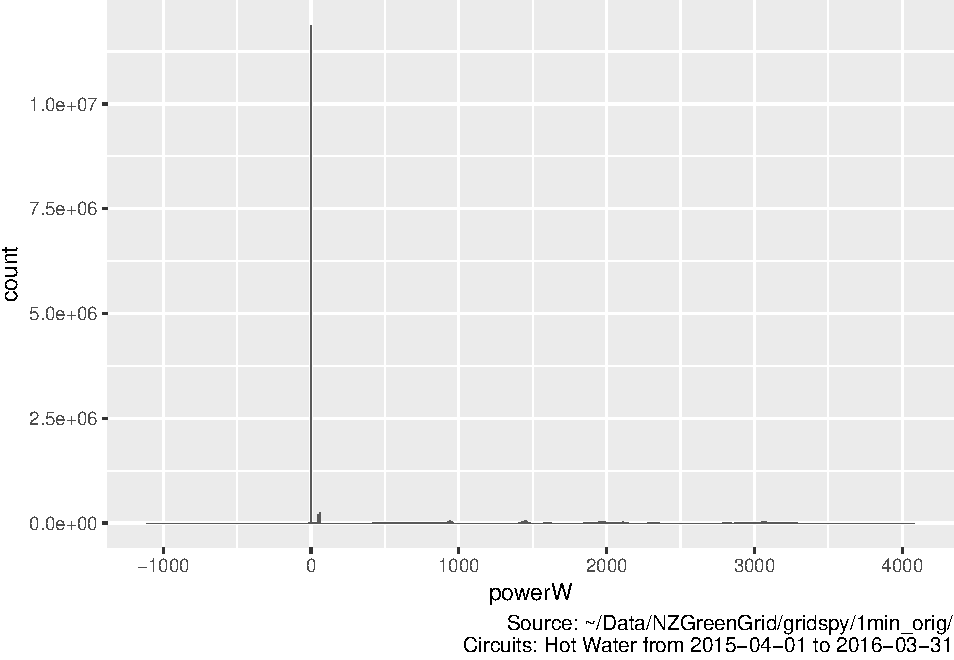
\includegraphics{ggHotWaterProfiles_files/figure-latex/histo full-1.pdf}

The next shows the histogram for powerW \textless{} 1000W\ldots{}

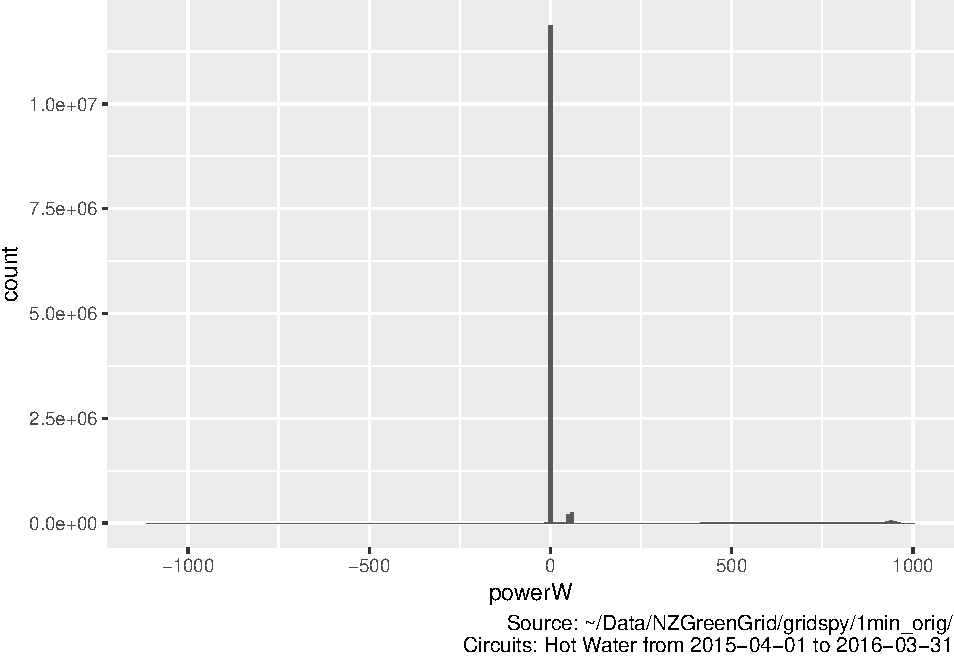
\includegraphics{ggHotWaterProfiles_files/figure-latex/histo power under 1000-1.pdf}

\begin{quote}
There are a lot of zeros (as we'd expect) but why are there negative
values?
\end{quote}

\section{Hot Water profiles}\label{hot-water-profiles}

This section produces the profiles as one for each HH but averaged over
each season. Data is kept at 1 minute intervals. Note definition of
season below\ldots{}

\begin{Shaded}
\begin{Highlighting}[]
\CommentTok{# add season}
\NormalTok{gs1MinDT <-}\StringTok{ }\NormalTok{gs1MinDT[, month }\OperatorTok{:}\ErrorTok{=}\StringTok{ }\NormalTok{lubridate}\OperatorTok{::}\KeywordTok{month}\NormalTok{(r_dateTime, }\DataTypeTok{label =} \OtherTok{TRUE}\NormalTok{)]}
\NormalTok{gs1MinDT <-}\StringTok{ }\NormalTok{gs1MinDT[, season }\OperatorTok{:}\ErrorTok{=}\StringTok{ "Summer"}\NormalTok{]}
\NormalTok{gs1MinDT <-}\StringTok{ }\NormalTok{gs1MinDT[, season }\OperatorTok{:}\ErrorTok{=}\StringTok{ }\KeywordTok{ifelse}\NormalTok{(month }\OperatorTok{==}\StringTok{ "Mar"} \OperatorTok{|}
\StringTok{                                              }\NormalTok{month }\OperatorTok{==}\StringTok{ "Apr"} \OperatorTok{|}
\StringTok{                                              }\NormalTok{month }\OperatorTok{==}\StringTok{ "May"}\NormalTok{, }\StringTok{"Autumn"}\NormalTok{, season)]}
\NormalTok{gs1MinDT <-}\StringTok{ }\NormalTok{gs1MinDT[, season }\OperatorTok{:}\ErrorTok{=}\StringTok{ }\KeywordTok{ifelse}\NormalTok{(month }\OperatorTok{==}\StringTok{ "Jun"} \OperatorTok{|}
\StringTok{                                              }\NormalTok{month }\OperatorTok{==}\StringTok{ "Jul"} \OperatorTok{|}
\StringTok{                                              }\NormalTok{month }\OperatorTok{==}\StringTok{ "Aug"}\NormalTok{, }\StringTok{"Winter"}\NormalTok{, season)]}
\NormalTok{gs1MinDT <-}\StringTok{ }\NormalTok{gs1MinDT[, season }\OperatorTok{:}\ErrorTok{=}\StringTok{ }\KeywordTok{ifelse}\NormalTok{(month }\OperatorTok{==}\StringTok{ "Sep"} \OperatorTok{|}
\StringTok{                                              }\NormalTok{month }\OperatorTok{==}\StringTok{ "Oct"} \OperatorTok{|}
\StringTok{                                              }\NormalTok{month }\OperatorTok{==}\StringTok{ "Nov"}\NormalTok{, }\StringTok{"Spring"}\NormalTok{, season)]}
\end{Highlighting}
\end{Shaded}

Profile plots:

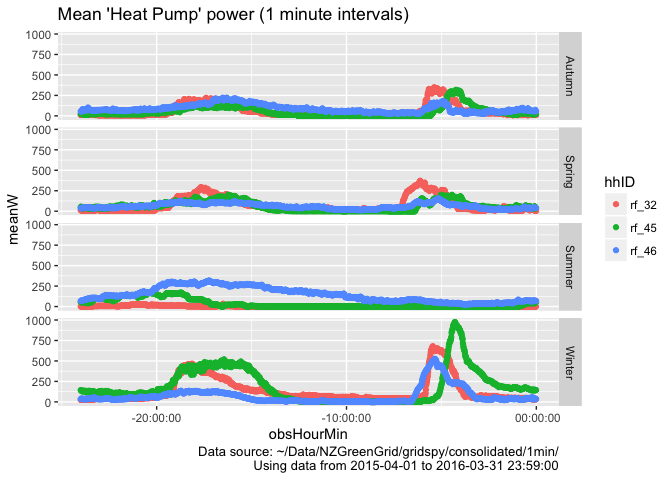
\includegraphics{ggHotWaterProfiles_files/figure-latex/profiles per household by season-1.pdf}

\begin{verbatim}
## [1] "Saving profile data used to build this plot to: /Users/ben/git.soton/ba1e12/nzGREENGrid/data/Hot Water_2015-04-01_2016-03-31_meanW_hhID_profiles_by_season.csv..."
\end{verbatim}

\begin{verbatim}
## [1] "Gzipped /Users/ben/git.soton/ba1e12/nzGREENGrid/data/Hot Water_2015-04-01_2016-03-31_meanW_hhID_profiles_by_season.csv"
\end{verbatim}

The plots could be repeated or re-facted e.g.~by household size.

Note that the code saves a high definition version of the chart and the
average profiles out to the repo (in
/Users/ben/git.soton/ba1e12/nzGREENGrid/data/Hot
Water\_2015-04-01\_2016-03-31\_meanW\_hhID\_profiles\_by\_season.csv.gz)
for future re-use.

The .csv.gz file can be loaded using the following code:

\begin{itemize}
\tightlist
\item
  \texttt{df\ \textless{}-\ readr::read\_csv("/Users/ben/git.soton/ba1e12/nzGREENGrid/data/Hot\ Water\_2015-04-01\_2016-03-31\_meanW\_hhID\_profiles\_by\_season.csv.gz")}
  or
\item
  \texttt{dt\ \textless{}-\ data.table::as.data.table(readr::read\_csv("/Users/ben/git.soton/ba1e12/nzGREENGrid/data/Hot\ Water\_2015-04-01\_2016-03-31\_meanW\_hhID\_profiles\_by\_season.csv.gz"))}
  if you prefer \href{}{data.table}
\end{itemize}

\section{Runtime}\label{runtime}

Analysis completed in 587.62 seconds ( 9.79 minutes) using
\href{https://cran.r-project.org/package=knitr}{knitr} in
\href{http://www.rstudio.com}{RStudio} with R version 3.5.0 (2018-04-23)
running on x86\_64-apple-darwin15.6.0.

\section{R environment}\label{r-environment}

R packages used:

\begin{itemize}
\tightlist
\item
  base R - for the basics (R Core Team 2016)
\item
  data.table - for fast (big) data handling (Dowle et al. 2015)
\item
  lubridate - date manipulation (Grolemund and Wickham 2011)
\item
  ggplot2 - for slick graphics (Wickham 2009)
\item
  readr - for csv reading/writing (Wickham, Hester, and Francois 2016)
\item
  dplyr - for select and contains (Wickham and Francois 2016)
\item
  progress - for progress bars (Csárdi and FitzJohn 2016)
\item
  knitr - to create this document \& neat tables (Xie 2016)
\item
  kableExtra - for extra neat tables (Zhu 2018)
\item
  nzGREENGrid - for local NZ GREEN Grid project utilities
\end{itemize}

Session info:

\begin{verbatim}
## R version 3.5.0 (2018-04-23)
## Platform: x86_64-apple-darwin15.6.0 (64-bit)
## Running under: macOS High Sierra 10.13.5
## 
## Matrix products: default
## BLAS: /Library/Frameworks/R.framework/Versions/3.5/Resources/lib/libRblas.0.dylib
## LAPACK: /Library/Frameworks/R.framework/Versions/3.5/Resources/lib/libRlapack.dylib
## 
## locale:
## [1] en_GB.UTF-8/en_GB.UTF-8/en_GB.UTF-8/C/en_GB.UTF-8/en_GB.UTF-8
## 
## attached base packages:
## [1] stats     graphics  grDevices utils     datasets  methods   base     
## 
## other attached packages:
## [1] kableExtra_0.9.0  knitr_1.20        readr_1.1.1       ggplot2_2.2.1    
## [5] dplyr_0.7.5       data.table_1.11.2 nzGREENGrid_0.1.0
## 
## loaded via a namespace (and not attached):
##  [1] Rcpp_0.12.17      cellranger_1.1.0  pillar_1.2.2     
##  [4] compiler_3.5.0    plyr_1.8.4        bindr_0.1.1      
##  [7] prettyunits_1.0.2 tools_3.5.0       progress_1.1.2   
## [10] digest_0.6.15     viridisLite_0.3.0 lubridate_1.7.4  
## [13] evaluate_0.10.1   tibble_1.4.2      gtable_0.2.0     
## [16] pkgconfig_2.0.1   rlang_0.2.0       rstudioapi_0.7   
## [19] yaml_2.1.19       bindrcpp_0.2.2    xml2_1.2.0       
## [22] httr_1.3.1        stringr_1.3.1     hms_0.4.2        
## [25] rprojroot_1.3-2   grid_3.5.0        tidyselect_0.2.4 
## [28] glue_1.2.0        R6_2.2.2          readxl_1.1.0     
## [31] rmarkdown_1.9     purrr_0.2.4       reshape2_1.4.3   
## [34] magrittr_1.5      backports_1.1.2   scales_0.5.0     
## [37] htmltools_0.3.6   rvest_0.3.2       assertthat_0.2.0 
## [40] colorspace_1.3-2  labeling_0.3      stringi_1.2.2    
## [43] lazyeval_0.2.1    munsell_0.4.3
\end{verbatim}

\section*{References}\label{references}
\addcontentsline{toc}{section}{References}

\hypertarget{refs}{}
\hypertarget{ref-progress}{}
Csárdi, Gábor, and Rich FitzJohn. 2016. \emph{Progress: Terminal
Progress Bars}. \url{https://CRAN.R-project.org/package=progress}.

\hypertarget{ref-data.table}{}
Dowle, M, A Srinivasan, T Short, S Lianoglou with contributions from R
Saporta, and E Antonyan. 2015. \emph{Data.table: Extension of
Data.frame}. \url{https://CRAN.R-project.org/package=data.table}.

\hypertarget{ref-lubridate}{}
Grolemund, Garrett, and Hadley Wickham. 2011. ``Dates and Times Made
Easy with lubridate.'' \emph{Journal of Statistical Software} 40 (3):
1--25. \url{http://www.jstatsoft.org/v40/i03/}.

\hypertarget{ref-baseR}{}
R Core Team. 2016. \emph{R: A Language and Environment for Statistical
Computing}. Vienna, Austria: R Foundation for Statistical Computing.
\url{https://www.R-project.org/}.

\hypertarget{ref-ggplot2}{}
Wickham, Hadley. 2009. \emph{Ggplot2: Elegant Graphics for Data
Analysis}. Springer-Verlag New York. \url{http://ggplot2.org}.

\hypertarget{ref-dplyr}{}
Wickham, Hadley, and Romain Francois. 2016. \emph{Dplyr: A Grammar of
Data Manipulation}. \url{https://CRAN.R-project.org/package=dplyr}.

\hypertarget{ref-readr}{}
Wickham, Hadley, Jim Hester, and Romain Francois. 2016. \emph{Readr:
Read Tabular Data}. \url{https://CRAN.R-project.org/package=readr}.

\hypertarget{ref-knitr}{}
Xie, Yihui. 2016. \emph{Knitr: A General-Purpose Package for Dynamic
Report Generation in R}. \url{https://CRAN.R-project.org/package=knitr}.

\hypertarget{ref-kableExtra}{}
Zhu, Hao. 2018. \emph{KableExtra: Construct Complex Table with 'Kable'
and Pipe Syntax}. \url{https://CRAN.R-project.org/package=kableExtra}.


\end{document}
